\section*{Microeconomics Midterm 2014 / 15}

{
\subsection*{Schmidt}

\subsubsection*{Exercise 1}

\begin{enumerate}[label=(\alph*)]
{\item 
\begin{align*}
    x_{1}(\lambda p, \lambda w)=\lambda^{1+\alpha-\delta} \frac{p_{1}^{\alpha} w}{p_{1}^{\delta}+p_{2}^{\delta}+p_{3}^{\delta}}=\lambda^{1+\alpha-\delta} x_{1}(p, w)
\end{align*}

Must have $1+\alpha-\delta=0$ or $\alpha=\delta-1$

\begin{align*}
    x_{2}(\lambda p, \lambda w)=\lambda^{1+\alpha-\delta} \frac{p_{2}^{\alpha} w}{p_{1}^{\delta}+p_{2}^{\delta}+p_{3}^{\delta}}+\beta \frac{p_{1}}{p_{3}} \frac{\lambda}{\lambda}
\end{align*}

No restriction on $\beta$.

\begin{align*}
    x_{3}(\lambda p, \lambda w)=\lambda^{1+\alpha-\sigma} \frac{\gamma p_{3}^{\alpha} w}{p_{1}^{\delta}+p_{2}^{\delta}+p_{3}^{\delta}}=\lambda^{1+\alpha-\delta} x_{3}(p, w)
\end{align*}

No restriction on $\gamma$.

In summary, we only need $\alpha=\delta-1$.
}
{\item 

\begin{align*}
    p_{1} x_{1}(\cdot)+p_{2} x_{2}(\cdot)+p_{3} x_{3}(\cdot) &= w \quad \text{to satisfy Walras' Law} \\
    \Leftrightarrow \frac{w}{p_{1}^{\delta}+p_{2}^{\sigma}+p_{3}^{\sigma}}\left[p_{1}^{1+\alpha}+p_{2}^{1+\alpha}+\gamma p_{3}^{1+\alpha}\right]+\beta \frac{p_{1} p_{2}}{p_{3}} &= w
\end{align*}

Must have $\beta=0$ :

\begin{align*}
    p_{1}^{\delta}+p_{2}^{\delta}+p_{3}^{\delta}=p_{1}^{1+\alpha}+p_{2}^{1+\alpha}+\gamma p_{3}^{1+\alpha}
\end{align*}

Must have $\gamma=1$ \& $\alpha=\delta-1$.

In summary:

\begin{align*}
    \alpha=\delta-1 \quad \beta=0 \quad \gamma=1
\end{align*}
}
\end{enumerate}
}
{
\subsubsection*{Exercise 2}

\begin{enumerate}[label=(\alph*)]
{\item 
Invert $e(p,u)$ as in equilibrium: $e(p, u)=w$ and also $u=v(p, w)$

\begin{align*}
    v\left(p, w\right)=w \frac{p_{1}+p_{2}}{p_{1} p_{2}}=w\left[\frac{1}{p_{1}}+\frac{1}{p_{2}}\right]
\end{align*}
}
{\item 
Roy's Identity

\begin{align*}
    x_1\left(p_1 w\right)=-\frac{\frac{\partial v(\cdot)}{\partial p_1}}{\frac{\partial v(\cdot)}{\partial w}}=\frac{w \frac{1}{p_1^2}}{\frac{p_1+p_2}{p_1 p_2}}=\frac{w}{p_1+p_2}\frac{p_2}{p_1} \\
    x_2\left(p_1 w\right)=\frac{w}{p_1+p_2} \frac{p_1}{p_2} \text { by symmetry }
\end{align*}
}
{\item 
\begin{align*}
    & \frac{x_1\left(p, w\right)}{x_2\left(p, w\right)}=\left(\frac{p_1}{p_2}\right)^{-2} \\
    & \eta_{12}=-(-2)\left(\frac{p_1}{p_2}\right)^{-3} \frac{\frac{p_1}{p_2}}{\left(\frac{p_1}{p_2}\right)^{-2}}=2
\end{align*}
}
\end{enumerate}
}
{
\subsubsection*{Exercise 2}

\begin{enumerate}[label=(\alph*)]
{\item 
Invert $e(p,u)$ as in equilibrium: $e(p, u)=w$ and also $u=v(p, w)$

\begin{align*}
    v\left(p, w\right)=w \frac{p_{1}+p_{2}}{p_{1} p_{2}}=w\left[\frac{1}{p_{1}}+\frac{1}{p_{2}}\right]
\end{align*}
}
{\item 
Roy's Identity

\begin{align*}
    x_1\left(p_1 w\right)=-\frac{\frac{\partial v(\cdot)}{\partial p_1}}{\frac{\partial v(\cdot)}{\partial w}}=\frac{w \frac{1}{p_1^2}}{\frac{p_1+p_2}{p_1 p_2}}=\frac{w}{p_1+p_2}\frac{p_2}{p_1} \\
    x_2\left(p_1 w\right)=\frac{w}{p_1+p_2} \frac{p_1}{p_2} \text { by symmetry }
\end{align*}
}
{\item 
CES utility:

\begin{align*}
    u\left(x_1, x_2\right)=\left[\frac{1}{2} x_1^\rho+\frac{1}{2} x_2^\rho\right]^{\frac{1}{\rho}} \text { where } \rho=1-\frac{1}{n_{12}}=1 / 2
\end{align*}
}
\end{enumerate}
}
{
\subsubsection*{Exercise 3}

The difference between consumer theory and production theory is mainly the fact that firms do not have budget constraints.
This problem introduces a budget constraint. Therefore, we are going to treat the problem like a consumer problem.
In that sense, the revenue is comparable to the utility function, and the cash constraint is like the wealth of a consumer.
Consequently, we are solving the following revenue maximization problem (which is the analogue to a utility maximization problem):

\begin{align*}
    \max_{z_1,z_2} pf(z_1,z_2) \\
    \operatorname{s.t.} \; w_1z_1 + w_2z_2 \leq C
\end{align*}

We will assume an interior solution (the budget constraint is binding).
Then, the revenue function $R(p, w_1, w_2, C)$ that the exercise gives us is just the equivalent to the indirect utility.

\begin{enumerate}[label=(\alph*)]
{\item 
As $R(p, w_1, w_2, C)$ works like the indirect utility, we apply Roy's identity to find the factor demand, which is the analogue to the Walrasian demand:

\begin{align*}
    z_1&=-\frac{\frac{\partial R}{\partial w_1}}{\frac{\partial R}{\partial C}} \\
    &= -\frac{p \cdot(-\alpha) \frac{1}{w_1}}{p \cdot \frac{1}{C}} \\
    &= \alpha \frac{C}{w_1}
\end{align*}
}
{\item 
We treat $R(p,w,C)$ as the indirect utility depending on income and invert it to find the cost function $C(p,w,R)$, which is the analogue to the expenditure function in consumer theory:

\begin{align*}
    R&=p\left[\gamma+\ln C(p,w,R)-\alpha \ln w_1-(1-\alpha) \ln w_2\right] \\
    \frac{R}{p}-\gamma &= \ln \left(\frac{C(p,w,R)}{w_1^\alpha w_2^{1-\alpha}} \right) \\
    \exp\left(\frac{R}{p}-\gamma\right)&=\frac{C(p,w,R)}{w_1^\alpha w_2^{1-\alpha}} \\
    C(p,w,R) &= w_1^\alpha w_2^{1-\alpha}\exp\left(\frac{R}{p}-\gamma\right)
\end{align*}
}
{\item 
Since the cost function from (b) happens to be the analogue to the expenditure function, we can apply Shephard's Lemma in order to find the factor demand for a given $R$ at minimum cost, as this is the analogue to the Hicksian demand in consumer theory.
In that spirit, let us call this function $h_1(p,w,R)$.

\begin{align*}
    h_1(p,w,R)&=\frac{\partial C\left(w,R\right)}{\partial w_1} \\
    &= \alpha \exp \left[\frac{R}{p}-\gamma\right] \cdot\left(\frac{w_2}{w_1}\right)^{1-\alpha}
\end{align*}
}
{\item 
In consumer theory, the Hicksian demand and the Walrasian demand meet at optimum. We can also show that here:

\begin{align*}
    h_1(w,R)&=z_1^* \\
    \alpha \exp \left[\frac{R}{p}-\gamma\right] \cdot\left(\frac{w_2}{w_1}\right)^{1-\alpha}&=\alpha \frac{C}{w_1}\\
    \exp \left[\frac{R}{p}-\gamma\right] w_1^\alpha w_2^{1-\alpha}&=C \\
    \frac{R}{p}-\gamma &= \ln \left(\frac{C}{w_1^\alpha w_2^{1-\alpha}} \right) \\
    R&=p\left[\gamma+\ln C-\alpha \ln w_1-(1-\alpha) \ln w_2\right]
\end{align*}

The last line is exactly the formula for the revenue that is observed by our econometrician friend in the optimum. Therefore, we have shown that the two demands are equal whenever the firm is acting optimally, i.e. maximizing its revenue or minimizing its cost. Put differently, the revenue maximization problem is the dual problem to the cost minimization problem and vice versa.
}
\end{enumerate}
}

\newpage
{
\subsection*{Gottardi}

\subsubsection*{Exercise 1}

\begin{enumerate}[label=(\alph*)]
{\item 
True. We need three things for FWT:

\begin{itemize}
    \item LNS, which is satisfied by monotonicity
    \item Complete markets, satisfied by two prices for two commodities
    \item free disposal (given)
\end{itemize}
}
{\item 
False. Convexity is violated by B. Consider the following illustration:

\begin{figure}[!h]
    \centering
    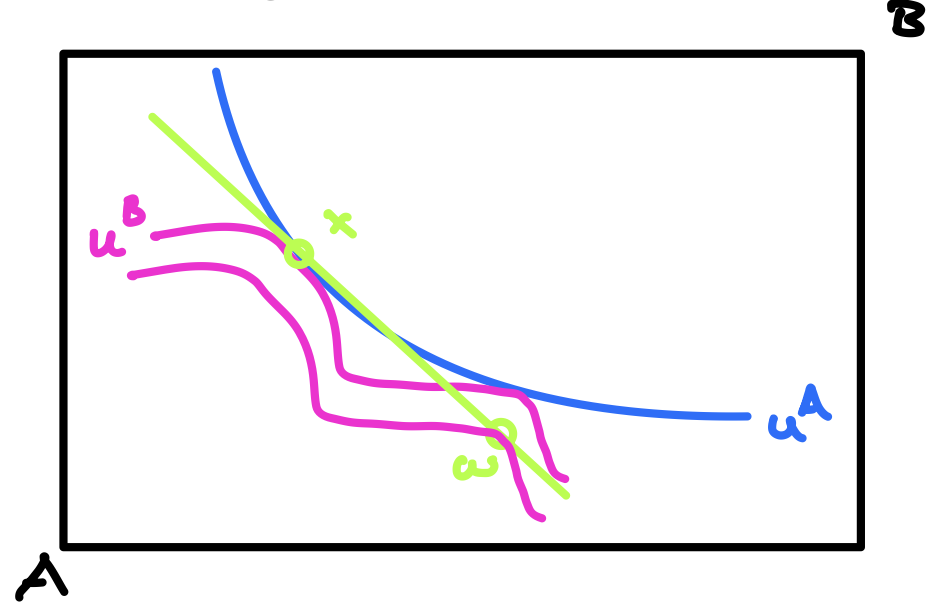
\includegraphics[width=0.75\linewidth]{images/2014_15_1.png}    
\end{figure}

Because $B$ has non-convex preferences, $x$ is not a CE. Actually no CE exists.
}
{\item 
False by same argument as in (b).
}
\end{enumerate}
}
{
\subsubsection*{Exercise 2}

\begin{enumerate}[label=(\alph*)]
{\item 
PE allocations are along $x_{1}^{A}=x_{2}^{A}$. If we are at any other point, just give some to $B$ because $A$ only cares about lower amount.

\begin{figure}[!h]
    \centering
    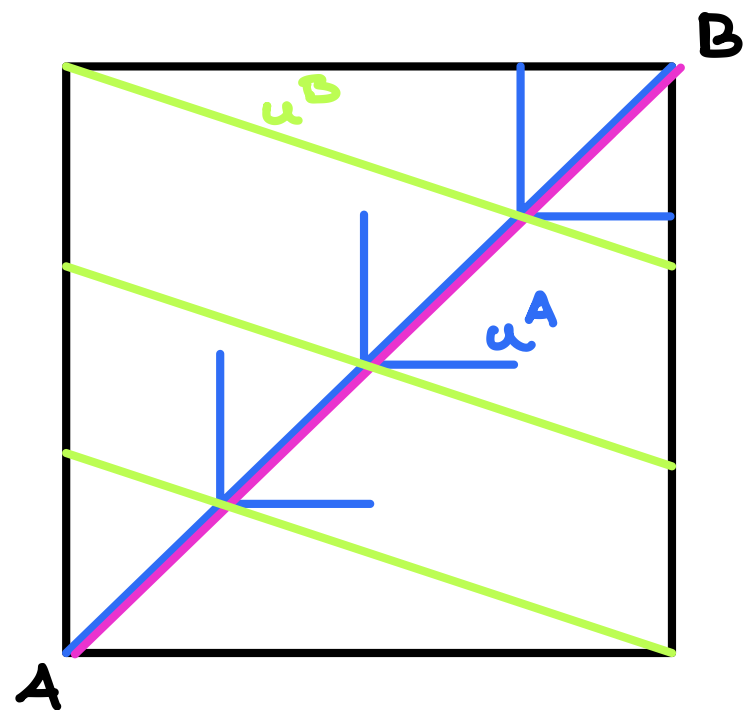
\includegraphics[width=0.75\linewidth]{images/2014_15_2.png}    
\end{figure}
}
{\item 
Let $p=\frac{p_{1}}{p_{2}}$

\underline{Consumer A:}

\begin{align*}
    x_{1}^{A}=x_{2}^{A} \quad\text{BC: } p x_{1}^{A}+x_{2}^{A}=6 p+2
\end{align*}

\underline{Consumer B:}

\begin{align*}
    x_1^B=\left\{\begin{array}{lll}
        \infty & \text { if } & p<1 / 3 \\
        \mathbb{R}^{+} & \text {if } & p=1 / 3 \\
        0 & \text { if } & \rho>1 / 3
    \end{array}\right. 
    \quad ; \quad
    x_2^B=\left\{\begin{array}{lll}
        \infty & \text { if } & p>1 / 3 \\
        \mathbb{R}^{+} & \text {if } & p=1 / 3 \\
        0 & \text { if } & p<1 / 3
    \end{array}\right. \\
    \text{BC: } p x_1^B+x_2^B=2 p+6
\end{align*}

\underline{Market Clearing:}

\begin{align*}
    & x_1^A+x_1^B = w_1^A+w_1^B=8 \\
    & x_2^A+x_2^B = w_2^A+w_2^B=8
\end{align*}

use $x_1^A=x_2^A \longrightarrow x_1^B=x_2^B$. Therefore $p=\frac{1}{3}$ so no excess demand for either good.

By $\operatorname{BC}^A$:

\begin{align*}
    & x_1^A=x_2^A=3 \\
    & x_1^B=x_2^B=5
\end{align*}

\underline{Competitive Equilibrium:}

\begin{align*}
    \left(x_1^A, x_2^A\right) & =(3,3) \\
    \left(x_1^B, x_2^B\right) & =(5,5) \\
    p & =\frac{1}{3}
\end{align*}

This is PE since $x_1^A = x_2^A$.
}
{\item 
Yes. The reason is that $p=\frac{1}{3}$ is the only possible equilibrium price. Otherwise markets cannot clear \& we have excess demand for one of the commodities.
}
\end{enumerate}
}
{
\subsubsection*{Exercise 3}

$w^1=(8,4) \text {; } \quad w^2=(2,6)$

\begin{enumerate}[label=(\alph*)]
{\item 
Note that we have (1) identical beliefs
and (2) no aggregate risk as $w_{1}=w_{2}=10$.

Therefore, full risk sharing is possible and $x_{1}^{h}=x_{2}^{h} \quad \forall h$ is PE. I.e. the $45^{\circ}$-line:

\begin{figure}[!h]
    \centering
    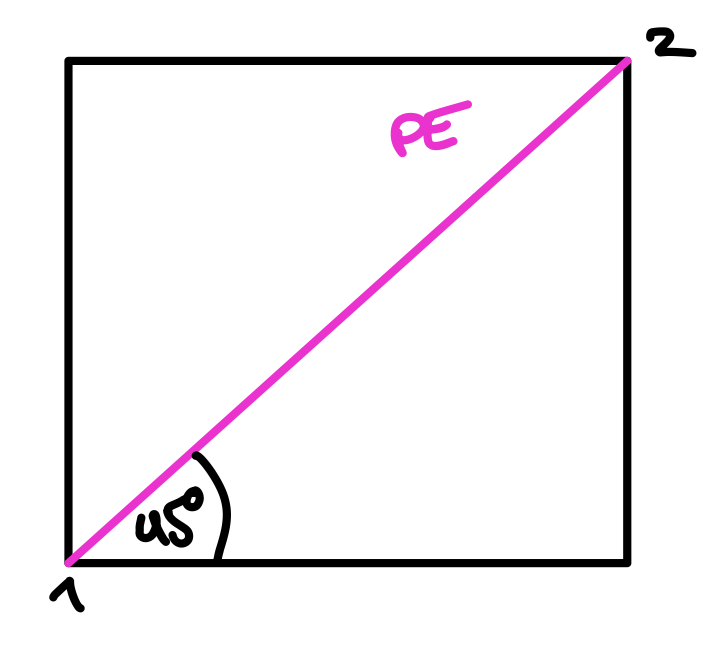
\includegraphics[width=.75\textwidth]{images/2014_15_3.png}
\end{figure}
}
{\item 
\underline{Consumer h:}

\begin{align*}
    \max_{x_{1}^{h}, x_{2}^{h}} \quad & \pi u^{h}\left(x_{1}^{h}\right)+(1-\pi) u^{h}\left(x_{2}^{h}\right) \\
    \text { s.t. } \quad & q_{1} \theta_{1}^{h}+q_{2} \theta_{2}^{h}=0 \\
    & x_{1}^{n}=w_{1}^{h}+\theta_{1}^{h} \\
    & x_{2}^{u}=w_{1}^{h}+\theta_{2}^{h}
\end{align*}

Plug in the $\theta$s:

\begin{align*}
    \max _{x_{1}^{h}, x_{2}^{h}} \quad & \pi u^{h}\left(x_{1}^{h}\right)+(1-\pi) u^{h}\left(x_{2}^{h}\right) \\
    \text { s.t. } & q_{1}\left(x_{1}^{h}-w_{1}^{h}\right)+q_{2}\left(x_{2}^{h}-w_{2}^{h}\right)=0
\end{align*}

FOCs:

\begin{align*}
    \pi \frac{\partial u^{h}\left(x_{1}^{h}\right)}{\partial x_{1}^{h}}-\lambda q_{1}&=0 \\
    (1-\pi) \frac{\partial u^{h}\left(x_{2}^{h}\right)}{\partial x_{2}^{h}}-\lambda q_{2} &= 0 \\
    \Longrightarrow \quad \frac{q_{1}}{q_{2}} &= \frac{\pi}{1-\pi} \frac{\frac{\partial u^{h}\left(x_{1}^{h}\right)}{\partial x_{1}^{h}}}{\frac{\partial u^{h}\left(x_{2}^{h}\right)}{\partial x_{2}^{h}}}
\end{align*}

Perfect risk sharing implies: $x_{1}^{h} = x_{2}^{h}$, and therefore we have 

\begin{align*}
    \frac{q_1}{q_2}=\frac{\pi}{1-\pi}
\end{align*}

Plug this into the BC:

\begin{align*}
    \frac{q_{1}}{q_{2}}\left(x_{1}^{h}-w_{1}^{h}\right)+x_{1}^{h}-w_{2}^{h} &= 0 \\
    x_{1}^{h}\left(\frac{q_{1}}{q_{2}}+1\right) &= w_{2}^{h}+w_{1}^{h} \frac{q_{1}}{q_{2}} \\
    x_{1}^{h}=x_{2}^{h}=\left(\frac{q_{1}}{q_{2}}+1\right)^{-1}\left(w_{2}^{h}+w_{1}^{h} \frac{q_{1}}{q_{2}}\right) 
    &= (1-\pi)\left(w_{2}^{h}+w_{1}^{h} \frac{\pi}{1-\pi}\right) 
    =\pi w_{1}^{h}+(1-\pi) w_{2}^{h} \\
    x_{1}^1=x_{2}^1 &= \pi 8+(1-\pi) 4=4(1+\pi) \\
    x_{1}^{2}=x_{2}^{2} &= \pi 2+(1-\pi) 6=6-4 \pi
\end{align*}

\underline{Competitive Equilibrium: }

\begin{align*}
    \left(x_1^1, x_2^1\right) & =(4+4 \pi, 4+4 \pi) \\
    \left(x_1^2, x_2^2\right) & =(6-4 \pi, 6-4 \pi) \\
    \frac{q_1}{q_2} & =\frac{\pi}{1-\pi}
\end{align*}
}
\end{enumerate}
}